% 导言区
\documentclass{article}%book ,report ,letter

\usepackage{graphicx}
\usepackage{xcolor}
\usepackage{listings}
\usepackage{fontspec}
\usepackage{setspace}
\usepackage{titlesec}
\setmonofont{Consolas}
\usepackage{ctex}%引入中文包,使得中文可以正常显示
\usepackage[left=2.5cm,right=2.5cm,top=2.0cm,bottom=2.0cm]{geometry}

\Huge{\title{\heiti 可视化数据结构演示项目 Dynamic Tree 设计报告}

\author{3170105785 杨溆峰 $\qquad$ 3170104169 连佳宜 $\qquad$ 3170104559 李举仁}

\date{2019年7月16日}

\begin{document}
	\maketitle
	\zihao{-4}
\section{问题背景}	
	\par 数据结构课程是大学计算机专业教育的核心课程,是实现各种复杂的成熟算法的核心基础。数据结构因其物理意义上的抽象性,往往难以进行十分合理的判断和预测,因此很多同学在理解数据结构的构建过程和运行过程上,往往存在一定的困难。同时,目前大多数老师在进行数据结构课程的讲授时,存在着 "照本宣科" 的现象,并没有对于各种数据结构进行充分的实例演示,这对于同学们理解数据结构的核心和内涵是不利的。这便是本次课程设计的出发点。
	\par 本课程设计针对普通的二叉搜索树,AVL Tree,以及 Splay Tree,完整地演示了它们的插入和删除过程,并且给出了查找一个点的功能,以及按照三种遍历顺序分别显示各个点的过程。由于 MVVM 开发模式的模块独立性和可扩展性,在本程序模块上扩展其他的数据结构也是容易的。本设计报告会阐明本程序考法过程中的小组分工,各轮迭代结果和最终测试结果。
	\par 项目源码仓库地址:https://github.com/Samsara-sd/dynamicTree
\section{开发计划和分工}
\subsection{开发计划}
	\par 本程序设计项目计划以 MVVM 模式进行开发,我们会对于先前使用 MVC 模式开发的暂时成品进行改写,预计会经过三轮迭代。在第一轮迭代结束之后,我们会搭建起 MVVM 的开发模式框架,并计划还原出关于 Binary Search Tree 的最简单的 Insert功能。二轮迭代结束后,我们希望已经基本还原三种数据结构的所有操作。而最后的三轮迭代,我们计划完成功能的进一步扩展,并进行 UI 界面的美化。具体的时间安排见下图。
	
\begin{figure}[htbp]
	\centering
	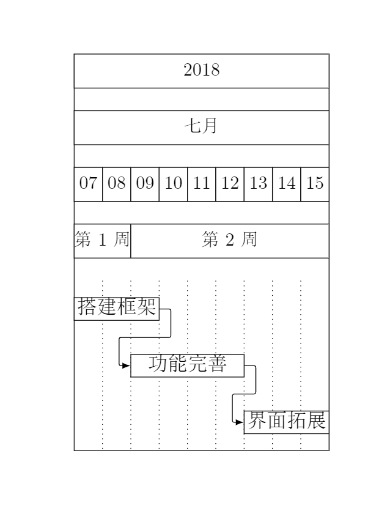
\includegraphics[height=8.0cm,width=7.0cm]{./image/7.png}
	\caption{开发计划和时间轴}
\end{figure}
	
\subsection{任务分工}
	\par 杨溆峰(3170105785): ViewModel 层的实现,持续集成工具部署,源代码仓库管理
	\par 连佳宜(3170104169): View 层和 App 层的实现,MVVM 框架的搭建,单元测试
	\par 李举仁(3170104559): Model 层和 Common 层的实现,代码覆盖率测试
\section{各轮迭代效果说明}
	\par 当改用 MVVM 模式进行开发之后,我们一共经历了三轮产品迭代,迭代后最终得到了最后的应用程序。接下来我们会对各轮迭代的效果进行说明。
\subsection{一轮迭代}
	\par 在一轮迭代结束之后,我们搭建起来了完整的 MVVM 开发框架,并还原出了普通的 Binary Search Tree 的 Insert 功能,且可视化演示部分也很好地实现了。
	
\begin{figure}[htbp]
	\centering
	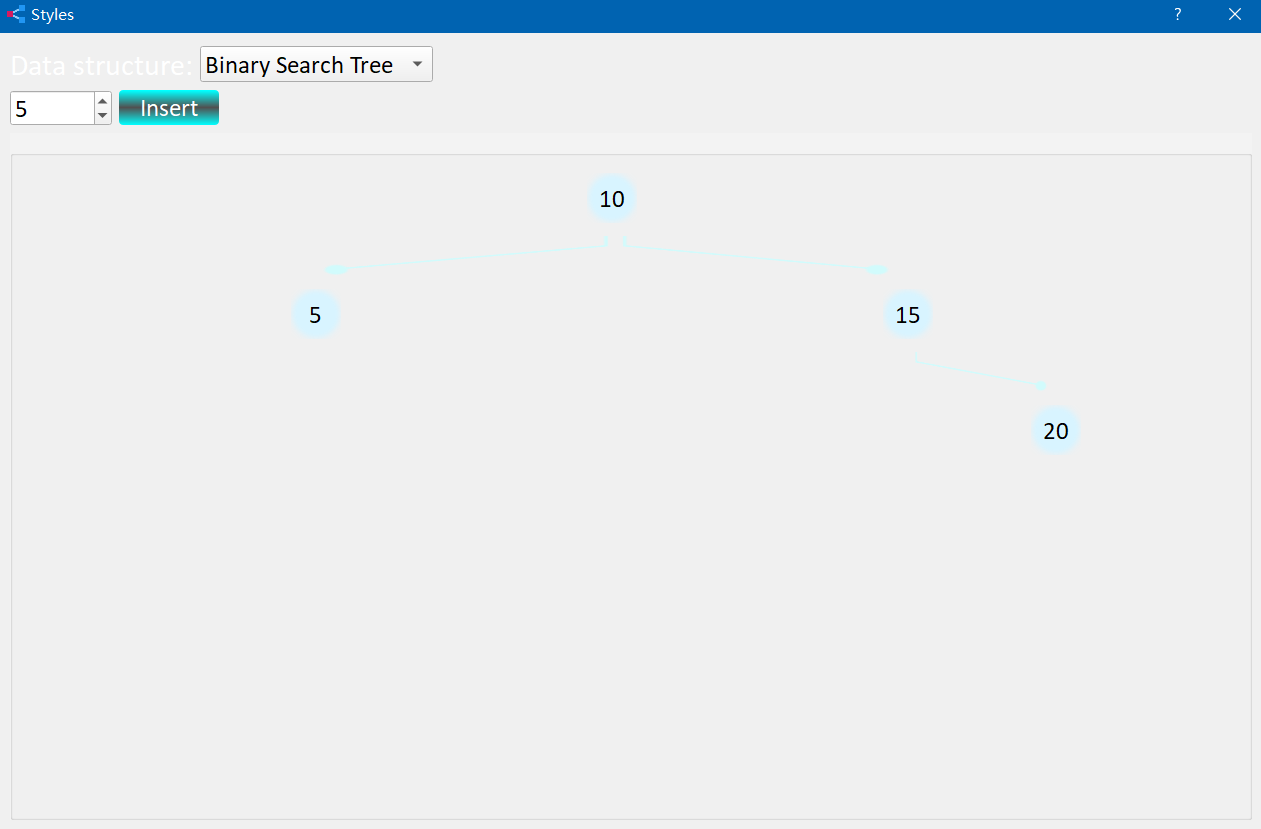
\includegraphics[height=8.0cm,width=12.0cm]{./image/8.png}
	\caption{一轮迭代结果}
\end{figure}	

\subsection{二轮迭代}
	\par 二轮迭代结束之后,我们还原了有关三种数据结构的所有基本操作(Insert, Delete, Find),并对他们的实际运行效果进行了充分的测试,发现在部分极端情况下会出现程序异常终止的情形,推测是逻辑方面的不完善导致了这样的结果。我们会在三轮迭代中进行进一步的完善。
	
\begin{figure}[htbp]
	\centering
	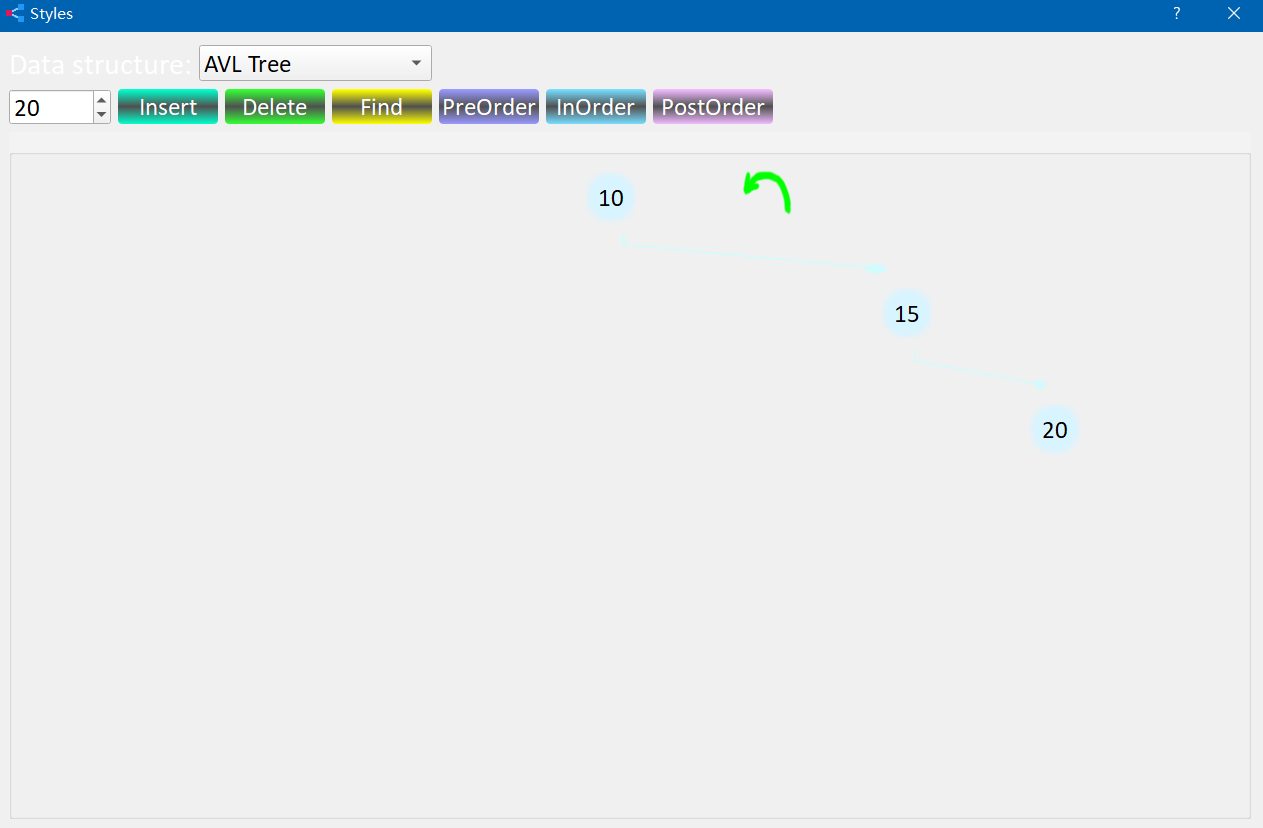
\includegraphics[height=8.0cm,width=12.0cm]{./image/9.png}
	\caption{二轮迭代结果}
\end{figure}	
	
\subsection{三轮迭代(终稿)}
	\par 在第三轮迭代中,功能方面我们对于 AVL Tree 自平衡操作和 Splay Tree 伸展操作的隐形 Bug 进行了修复,具体包括解决了 AVL Tree 在旋转操作时对子树平衡系数进行更新存在错误的问题,解决了 Splay Tree 的 Find 操作进行返回时存在的空指针问题等等。同时,我们还进行了 UI 界面的美化,并添加了 Choosefile 功能(从文件中读取一定量的整数并进行顺序插入)。本轮迭代的最终效果见下方的最终运行效果的演示。
\section{最终运行效果}
	\par 最终的项目消除了在前两轮迭代中发现的漏洞,并对于整体的 UI 界面进行了美化,并且通过时钟计时,延时设置等相关操作,使数据结构的每一步运行结果都可以缓慢变化进行演示,可以完整地,容易理解地展示出数据结构更新的整个过程。

\begin{figure}[htbp]
	\centering
	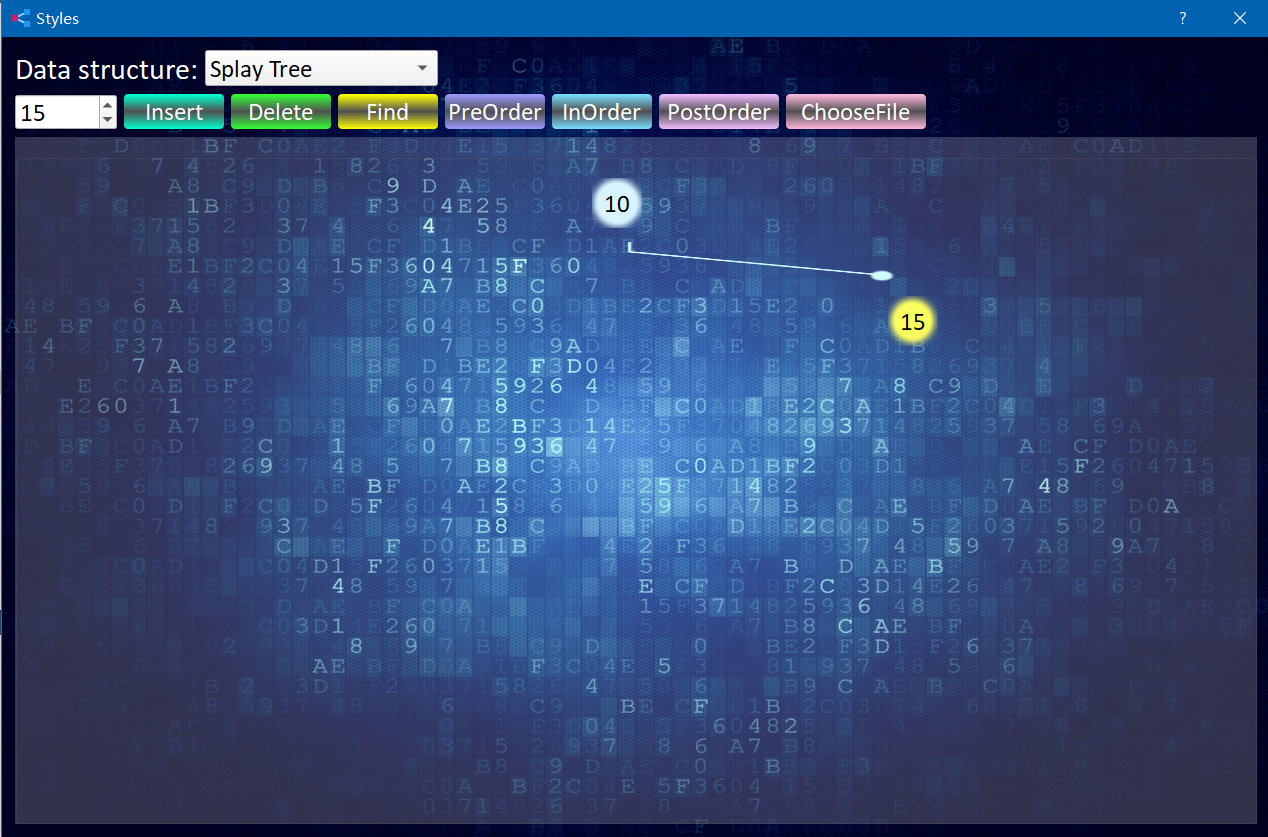
\includegraphics[height=6.0cm,width=8.0cm]{./image/1.png}
\end{figure}

\begin{figure}[htbp]
	\centering
	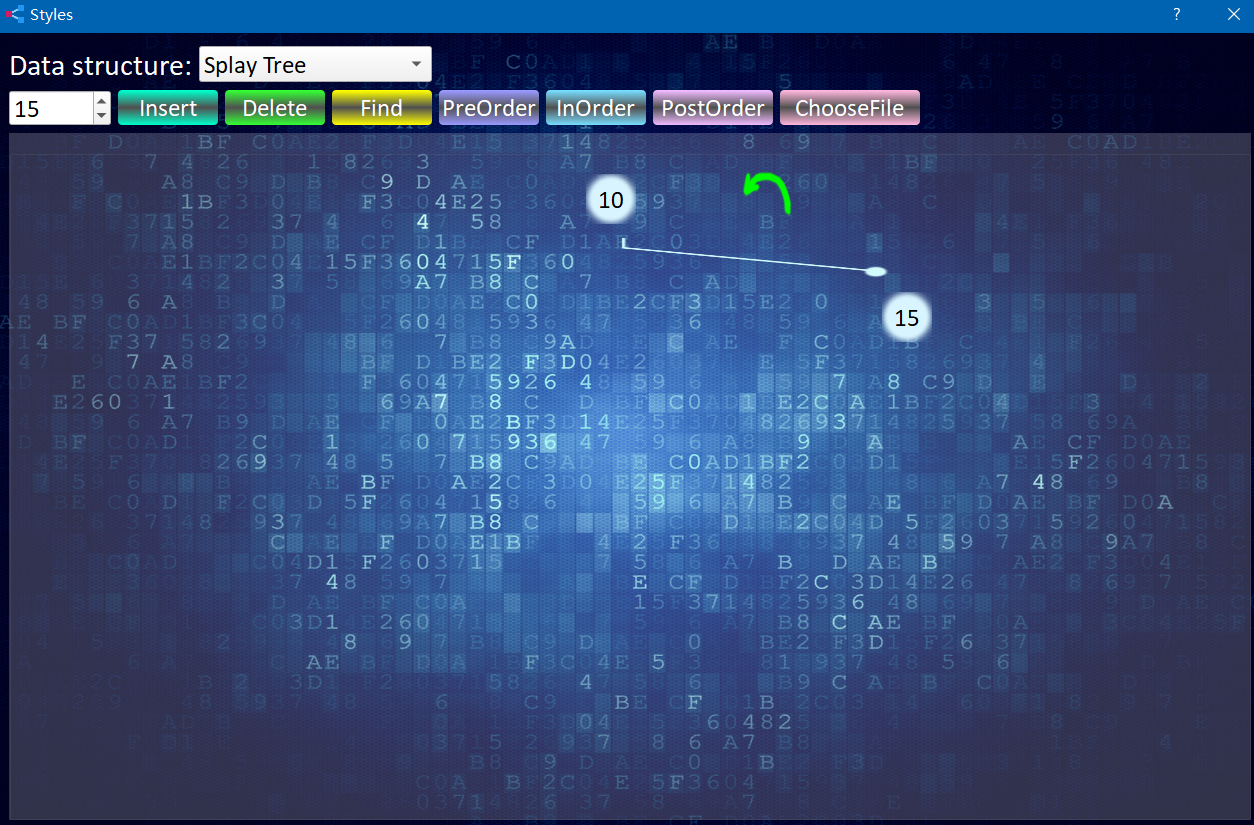
\includegraphics[height=6.0cm,width=8.0cm]{./image/2.png}
\end{figure}

\begin{figure}[htbp]
	\centering
	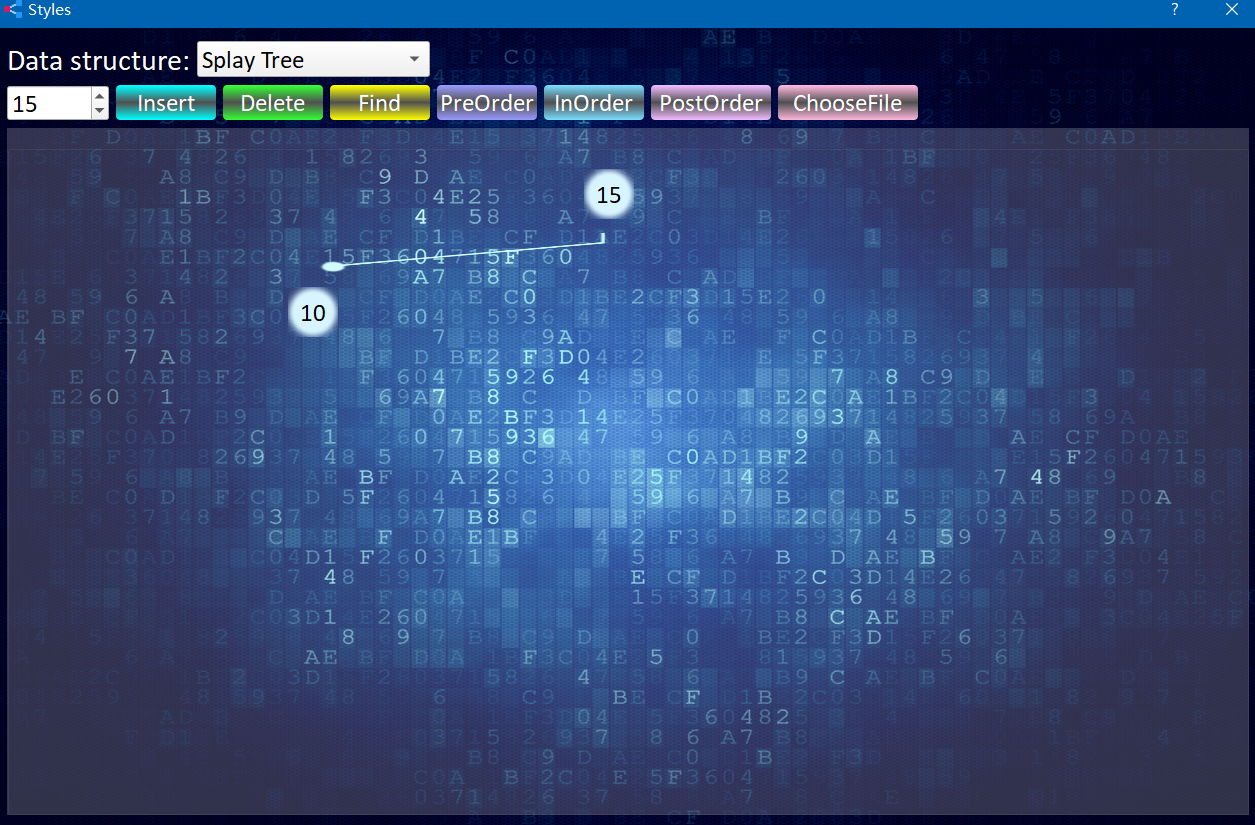
\includegraphics[height=6.0cm,width=8.0cm]{./image/3.png}
\end{figure}

\section{单元测试和代码覆盖率测试}
	\par 在最后的测试环节,我们编写了如下的 test 程序,其中的操作囊括了涉及三种树的所有种类的操作(插入,删除,寻找,顺序遍历),并且通过异常处理机制来寻找可能存在的有问题的操作。通过这一程序,我们结合 OpenCppCoverage 工具来进行代码覆盖率的测试,观察正常的对于三棵树的操作是否能够覆盖我们编写的所有功能模块。
\begin{spacing}{0.9}
	\begin{lstlisting}[language = C++, numbers=left, 
	numberstyle=\tiny,keywordstyle=\color{blue!70},
	commentstyle=\color{red!50!green!50!blue!50},frame=shadowbox,
	rulesepcolor=\color{red!20!green!20!blue!20},basicstyle=\ttfamily]
// ViewModelTest.cpp
#include "ViewModelTest.h"
#include "../common/etlbase.h"
#include "../viewmodel/viewmodel.h"
#include "../model/model.h"
std::shared_ptr<ViewModelClass> vmdl(std::make_shared<ViewModelClass>());
std::shared_ptr<ModelClass> model(std::make_shared<ModelClass>());

void Test_BST()
{
    bool bRet = vmdl->modelInsert(20);
    if( !bRet )
        throw int(1);
    bRet = vmdl->modelInsert(15);
    if( !bRet )
        throw int(1);
    bRet = vmdl->modelInsert(25);
    if( !bRet )
        throw int(1);
    bRet = vmdl->modelInsert(12);
    if( !bRet )
        throw int(1);
// ······
}

bool ViewModel_Test() throw()
{
    try {
        vmdl->SetModel(model);
        //change Data Structure
        std::string Data_Structure = "Binary Search Tree";
        bool bRet = vmdl->modelChangeMode(Data_Structure);
        if( !bRet )
            throw int(4);
        Test_BST();
        //change Data Structure
        Data_Structure = "AVL Tree";
        bRet = vmdl->modelChangeMode(Data_Structure);
        if( !bRet )
            throw int(4);
        Test_AVL();
        //change Data Structure
        Data_Structure = "SPlay Tree";
        bRet = vmdl->modelChangeMode(Data_Structure);
        if( !bRet )
            throw int(4);
        Test_SPlayTree();
        //Pre Order
        bRet = vmdl->modelPreOrder();
        if( !bRet )
            throw int(11);
        //In Order
        bRet = vmdl->modelInOrder();
        if( !bRet )
            throw int(12);
        //Post Order
        bRet = vmdl->modelPostOrder();
        if( !bRet )
            throw int(13);
    } catch (int& v) {
        printf("case %d error\n", v);
        return false;
    } catch (...) {
        printf("exception\n");
        return false;
    }
    return true;
}	
	\end{lstlisting}
\end{spacing}	
	$\,$
	\par 最后的测试结果可见项目根目录下的 Coverage Report 文件夹。文件夹下生成了针对工程源代码的每个 cpp 文件的代码覆盖测试的结果,由测试结果可见常用的功能基本上覆盖了我们编写的功能模块的所有情况。
	
\end{document}